\chapter{Background}\label{ch:Background}

This chapter will go through the necessary and interesting genomic biology aspects of the algorithm, for the reader to better understand the implications of the research.
It is meant for readers with little or no biological background, and as such it will start from the basics.
Then, a discussion of algorithms that have come before this thesis is made such that the algorithm introduced and its improvements are put into perspective.

\section{Biology Primer}\label{sec:Biology}

This section will start with an introduction to the natural aspect of biology, including what DNA is and how it can be analysed.
Genomic biology is a wide topic, hence this thesis will stick to what is relevant for it.
Later, this will be linked to how researchers can use sequencing technologies in order to make new inferences.

First is a description of what Deoxyribonucleic Acid (DNA) is.
Each organism is made up of cells, and each cell has different components, but in the center is a nucleus which is the driver of everything else, and within this nucleus is the DNA~\cite{CellBiology}.\@
The actual biology is more complicated than this, however, this is as far as the reader needs to understand about the cell structure.

The DNA contains a sequence of bases: Adenine, Cytosine, Thymine, and Guanine.
For the representation in this thesis, each base is represented by a single character: $ACGT$, corresponding to the first letter of the name of each base.
Each base has a pair, where the bases $A$ and $T$ bind together, and $C$ and $G$ also bind together.
These base pairs then attach to a sugar phosphate backbone to form the double helix of the DNA~\cite{DNA}.
Figure~\ref{fig:DoubleHelix} shows the different parts of the double helix visually.
Note that this representation is usually represented as a twisted ladder, but for clarity, a straightened ladder was chosen for the visualisation.

\begin{figure}[t]
  \centering
  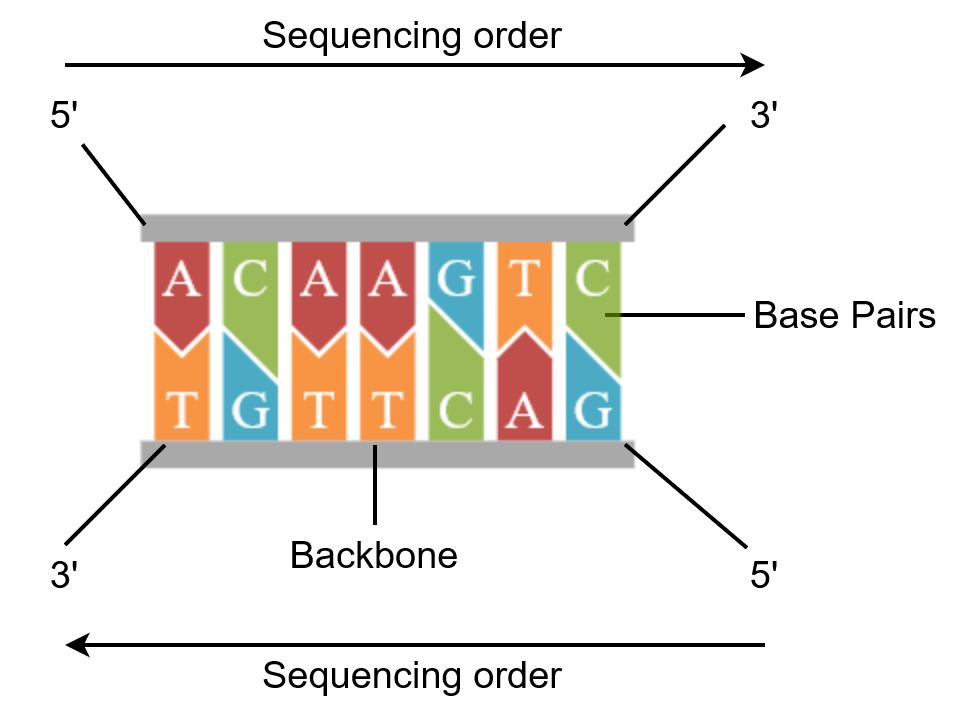
\includegraphics[width=0.55\textwidth]{images/DoubleHelix.png}
  \caption{The double helix of the DNA showing the 2 backbones and the attached base pairs. The visualisation was created using \url{https://www.petercollingridge.co.uk/tools/draw-dna/}}\label{fig:DoubleHelix}
\end{figure}

It is unfortunately very difficult to sequence an entire DNA strand at one go with current technologies.
Instead, a DNA of a sample is cloned multiple times, fractured, and read fragment by fragment~\cite{ShotgunSequencing}.
A sample may have multiple cells from different species, thus having multiple different DNA genomes jumbled together.
Sequencing can either be done using shotgun sequencing~\cite{ShotgunSequencingOriginal}, where each part of the DNA strand has an equal chance of appearing in the dataset, or targeted sequencing~\cite{TargetedSequencing}, where only certain parts of the DNA strand are targeted.
A single fragment is called a read.
The two types of this sequencing are short read sequencing (SRS) and long read sequencing (LRS)~\cite{SrsVsLrs}.
Longer reads are of course preferable because researchers can see more of a genome at a time, whereas with shorter reads, constructing a genome, which is discussed in Section~\ref{sec:DBG}, takes much longer due to the need for assembling many more reads together.
A genome is the full DNA string of a cell of an organism.
However, SRS is currently much more accurate than LRS~\cite{LrsChallenges}.
Accuracy in this case means that the sequenced bases are correct, and an error might be a base-flip, where, for example, an $A$ may be sequenced as a $C$.
Other sources of errors may be missing bases or the addition of non-existent bases.
Cost is also a big factor.
Two big players in these fields are Oxford Nanopore\footnote{\url{https://nanoporetech.com/}}, which perform LRS, and Illumina\footnote{\url{https://www.illumina.com/}}, which perform SRS and were the first to drop the cost of sequencing the full human genome to under \$1000~\cite{LrsChallenges}.
Illumina have been around for almost 20 years now, and have taken a large market share since lots of algorithmic pipelines are based on their technology~\cite{SrsVsLrs}.

To read the DNA, a messenger RNA (mRNA) is used~\cite{mrna} in a method called transcription.
This reads a single strand of the DNA and, luckily, nature has evolved such that the strands are always read from the 5' (five prime) end to the 3' end, as visualised in Figure~\ref{fig:DoubleHelix}.
This means that researchers have more information on the direction of the read, though one still can not know from which of the two strands the read comes from.
A technique that is often used is to also consider the reverse complement of a read.
The reverse complement of a read is the whole string reversed and the bases replaced by their pairs~\cite{ReverseComplements}.
From Figure~\ref{fig:DoubleHelix}, the first strand of the read may be \textit{ACAAGTC}, whereas the reverse complement is \textit{GACTTGT}.\@
Note that both strings may be sequenced with equal probability and it is not possible to know from which strand each string originates from just by looking at the two of them.
One would need to assemble them with other reads in order to know where they belong.

De novo assembly is when different reads are combined together using overlaps in their prefixes and suffixes to construct the full reference genome~\cite{DeNovoAssembly}.
The na\"ive algorithm for this process is to try out all combinations of read pairs and positions and see where they fit best within the context of the whole genome, without knowing what the genome actually looks like~\cite{EulerianPath}.

Ideally, every cell in a body would have the same DNA sequence.
However, mutations do exist, and mutations also develop over time and inevitably lead to aging.
However, many mutations across different parts of the body may lead to severe diseases~\cite{Mutations}.
Hence, analysing these mutations within a genome is one use case for how researchers can use such DNA data and alignment techniques in order to find out more about, for example, the condition of a patient.

To analyse these mutations, alignment can then be used, after a reference genome has been constructed, where the reads of a new specimen are aligned to this genome.
Alignment means to find the best position within the reference genome where there are the least differences between the sequences~\cite{Alignment}.
Gaps may also occur when certain types of mutations occur, and they may also manifest themselves as a character flip within the DNA string.
One use case of alignment could be to find these mutations in the genetic code between healthy people and those with a certain disease, such as forms of cancer~\cite{BreastCancer}.
Figure~\ref{fig:Alignment} shows an example of two aligned reads with some differences.

\begin{figure}[t]
  \centering
  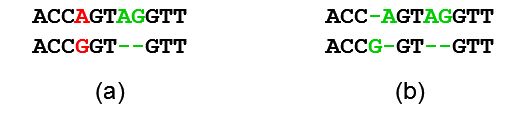
\includegraphics[width=0.55\textwidth]{images/Alignment.png}
  \caption{Two reads aligned to one another. Note that (a) and (b) represent the same two reads, but in one representation the first difference is represented  as a character flip, in red. Meanwhile, in (b) it is represented as 2 separate insertion and deletions in green. Gaps are represented with the '-' character. Since the reference genome is not known in this case, the second difference may be either an insertion or a deletion, or a mixture of both. When doing assembly, these sequences would instead be correlated with more reads to check their correctness and increase the confidence in the accuracy, rather than being compared to the reference genome. If this is all the information that was available, option (a) would be the preferred option to choose as there are fewer operations to align the two sequences.}\label{fig:Alignment}
\end{figure}

Contigs are also explained as they will be a useful concept in Section~\ref{sec:DBG}, mostly unitigs are discussed.
A contig forms when a set of reads is assembled together.
The assembled sequence from end to end is called a contig.
The term \textit{contig} comes from the word \textit{contiguous}, as the reads in the contig set are contiguous~\cite{Contig}.
This contig might contain some uncertainties, due to the mutations described previously.
Figure~\ref{fig:AssemblyAndAlignment} shows a more complex example of alignment with contigs.

\begin{figure}[t]
  \centering
  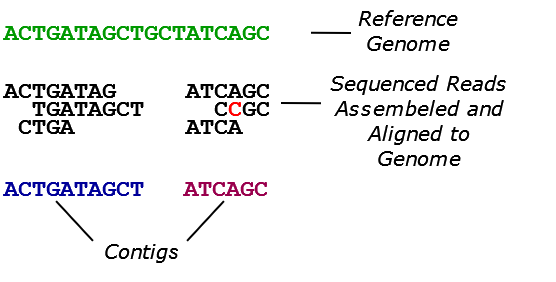
\includegraphics[width=0.55\textwidth]{images/AssemblyAndAlignment.png}
  \caption{A more complex diagram of alignment and assembly. The reference genome is given in green at the top, with the newly sequenced reads, assembled and aligned to the reference genome, in the middle, and the contigs extracted from those reads at the bottom. Note that if the reference genome was not known, then this would be doing De novo assembly, rather than alignment, to try to construct the genome without knowing it.}\label{fig:AssemblyAndAlignment}
\end{figure}

The data is stored in what are known as FASTA and FASTQ files.
An example of the FASTA format may be seen in Figure~\ref{fig:FASTA}.
This format consists of multiple sequences, each starting with the '>' character, followed by the title of the sequence, which is then followed by the sequence itself on the next line.
This sequence can be on multiple lines~\cite{FastaAndFastq}.
Besides the ACGT characters, which are sometimes in uppercase and other times in lowercase, the character N is sometimes used to signal an ambiguous base\footnote{\url{https://knowledge.illumina.com/software/general/software-general-reference_material-list/000003560}}.
The sequences may be genomes or reads.

The second file format is FASTQ, which contains additional information about the quality of each base in the read~\cite{FastaAndFastq}.
An example can be found in Figure~\ref{fig:FASTQ}.
This format starts with the '@' character followed by the title, and the read on the next line which can be of multiple lines similar to the FASTA format.
Then a '+' is added on the next line, which may or may not be followed by the same title of the sequence on the same line, and lastly the quality string on the next line (or lines) which should be of equal length as the sequence.
The characters of the quality string indicate the confidence in the corresponding base at that same index within the sequence.
The specifics of how these characters are interpreted will not be delved into, as they are not relevant to the rest of the text.

FASTA files are usually used for representing reference genomes, while FASTQ files are used for raw read data since they can also contain the quality string.
Unfortunately there is not a single standard for the file formats, although there are some attempts at creating some\footnote{\url{https://www.ncbi.nlm.nih.gov/genbank/fastaformat/}}.
Even the titles themselves can be of any form, as can be seen in the two examples.
The characters used for the quality string are also different between standards.
As such, writing a parser for these file formats can be a headache~\cite{FastaAndFastq}.
For this thesis, a scalable parser capable of supporting both FASTA and FASTQ files, or a mixture of both, was implemented, which is also capable of reading zipped and unzipped files.
This parser skips over title lines and quality strings, since these are not needed for this use case.

\begin{figure}
\centering
\begin{lstlisting}[basicstyle=\footnotesize\ttfamily]
>ERR345345.239 AJIJSDIO
ATCGTCACTAGCTAGCTAGCTACcagagctagtcagctagcactcagtcat
GCTCGAGTCAGC
>seq2
gtagcatcGATCGATCAGTGACNNNNNNNNNNNNNATGTCGAAAGAATAGTCGATG
CGATagtacgctcacgtacgactcgtc
>seq3
GAGTGAGTGCCCCtttaagagtattgtaGT
\end{lstlisting}
\caption{An example of a FASTA file with 3 sequences.}\label{fig:FASTA}
\end{figure}

\begin{figure}
\centering
\begin{lstlisting}[basicstyle=\footnotesize\ttfamily]
@ERR345345.239 AJIJSDIO
ATCGTCACTAGCTAGCTAGCTACcagagctagtcagctagcactcagtcat
GCTCGAGTCAGC
+ERR345345.239 AJIJSDIO
>)II8123))II328947289BA@@@@FFFFDFHFFHGHIGGGBFFAFGCF
;<B;@A5;5<DD
@seq2
gtagcatcGATCGATCAGTGACNNNNNNNNNNNNNATGTCGAAAGAATAGTCGATG
CGATagtacgctcacgtacgactcgtc
+
>)II8123))II328947289BA@@@@FFFFDFHFFHGHIGGGBFFAFGCF3))II
;<B;@A5;5<DD3))II3))II3))II
@seq3
GAGTGAGTGCCCCtttaagagtattgtaGT
+
@@@FFFFDFHFFHGHIGGGBFFAFGCF3))
\end{lstlisting}
\caption{An example of a FASTQ file with 3 sequences.}\label{fig:FASTQ}
\end{figure}

In the next sections, advancements in computer science algorithms will be discussed, which have made the analysis of such data more feasible and accurate.


\section{De Bruijn Graphs}\label{sec:DBG}

The first concept to introduce in this section will be that of the De Bruijn Graph (DBG)~\cite{DeBruijnGraph}, which are used throughout much of bioinformatics.
However, first some notation must be presented.
A graph $G=\{V,E\}$ consists of a set of vertices $V=\{v_1,v_2,\ldots,v_n\}$ which are connected by a set of edges $E=\{e_1, e_2, \ldots, e_m\}$.
The terms nodes and vertex will be used interchangeably.
Each vertex $v_i$ has a label $label(v_i)$, a set of outgoing nodes $out_v(v_i)$ of size $\#out_v(v_i)$, a set of incoming nodes $in_v(v_i)$ of size $\#in_v(v_i)$, a set of outgoing edges $out_e(v_i)$, and a set of incoming edges $in_e(v_i)$, of sizes with the same notation as the vertices.
Then, $v_1$ has an outgoing edge to $v_2$ if there exists an edge $e$ such that $e=v_1 \rightarrow v_2$.
Each edge $e_i$ also has a label $label(e_i)$.

To construct the DBG, the dataset must be transformed.
Given a set of FASTA and FASTQ files, all the sequences must first be extracted individually, and then, using a sliding window method, extract all unique substrings of a set size $k$.
These substrings are called $k$-mers, historically introduced as \textit{k-tuples}~\cite{DeBruijnGraph}.
Formally, given a sequence $S=[c_0, c_1, \ldots, c_{C-1}]$ of size $C$, a set of sequences $\{ [c_0,c_1,\ldots,c_{k - 1}], [c_1, c_2,\ldots,c_{k}], \ldots , [c_{C-k}, c_{C-k+1}, \ldots, c_{C - 1}]\}$ is extracted.
Often, the reverse complements of these $k$-mers are also computed and added to the set of unique $k$-mers.
For this reason, the size of $k$ is usually taken to be an odd number, in order to avoid palindromes between the forward and backwards sequence which can cause problems for some analysis tasks~\cite{Palindromes}.
An example of a palindrome may be \textit{AGCGCT}, where the reverse complement of this sequence would be itself.

Now graph construction may commence.
Given a pair of $k$-mers with sequences $S_0=[a_0, a_1, \ldots, a_{k - 1}]$ and $S_1=[b_0, b_1, \ldots, b_{k - 1}]$, one must first create the nodes $v_0$ and $v_1$ for these $k$-mers and give them the labels $S_0$ and $S_1$ respectively.
Then if the $k-1$ suffix of $S_0$ is equal to the $k-1$ prefix of $S_1$, that is, $[a_1, a_2, \ldots, a_{k - 1}] = [b_0, b_1, \ldots, b_{k-2}]$, create an edge $v_0 \rightarrow v_1$.
The labels of the edges are the character that is added in order to get to the next $k$-mer, that is, the final character of the outgoing node $v_1$, which is $b_{k - 1}$.
This is done for all $k$-mers which share a $k+1$ suffix and prefix.
Figure~\ref{fig:FastaqToDbg} shows an example of the whole pipeline from the FASTA/FASTQ files to a DBG.\@

\begin{figure}[t]
  \centering
  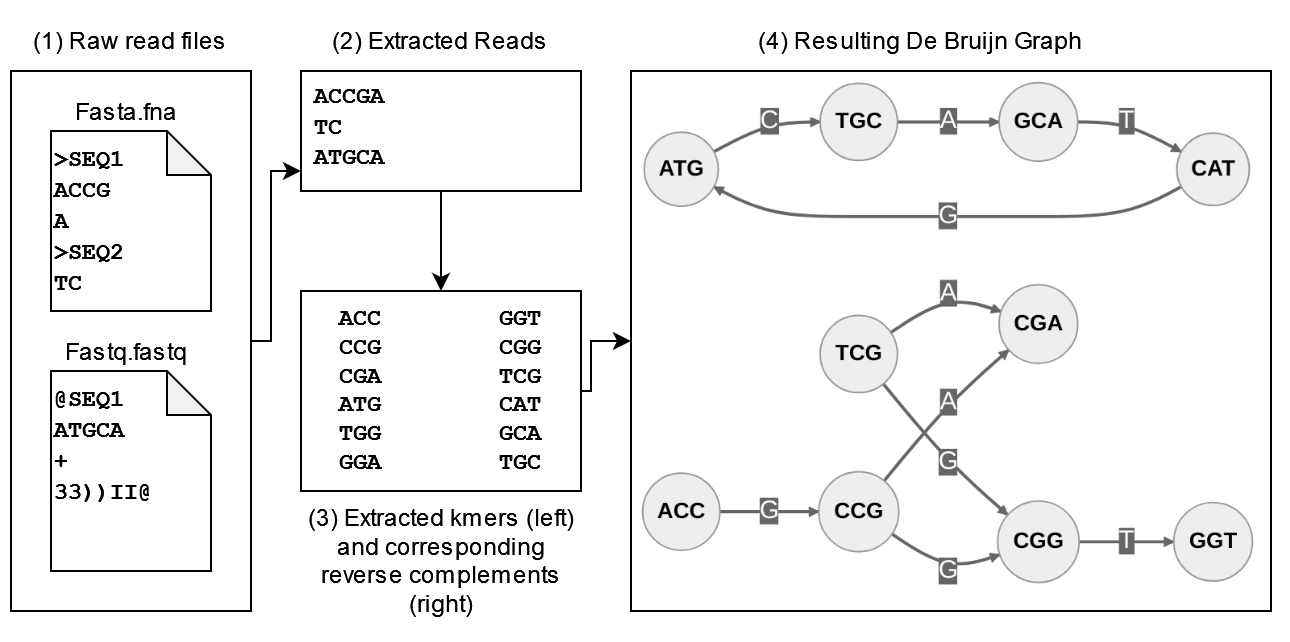
\includegraphics[width=\textwidth]{images/FastaqToDbg.png}
  \caption{The pipeline from FASTA/FASTQ files to the final DBG with $k = 3$.}\label{fig:FastaqToDbg}
\end{figure}

The DBG is a crucial part of many genome analysis tasks.
For example, it can be used to assemble a new genome by traversing it, and if there is a single Eulerian path for the entire graph, then it is known that this is the order in which reads must be assembled~\cite{DeBruijnGraph}.
An Eulerian path is a path that traverses all edges exactly once.
Note that this would not work for the graph in Figure~\ref{fig:FastaqToDbg}, but Figure~\ref{fig:EulerianPath} shows a good example of this.
That said, even this example may not be perfect, because the graph also consists of an unknown number of repeats.
Much work has been done to improve on assembly techniques of new genomes based on this method, especially tackling ambiguity issues when a single Eulerian path might not be possible, such as by giving more weight to certain nodes when they meet certain conditions~\cite{DeBruijnGraph, EulerianPath}.
Some readers may have already started thinking of ways to tackle the many potential challenges of such a problem~\cite{ModernAssembly}, however, this text will not be going into more detail about these assembly methods as they are not relevant to the rest of the contents.

\begin{figure}[t]
  \centering
  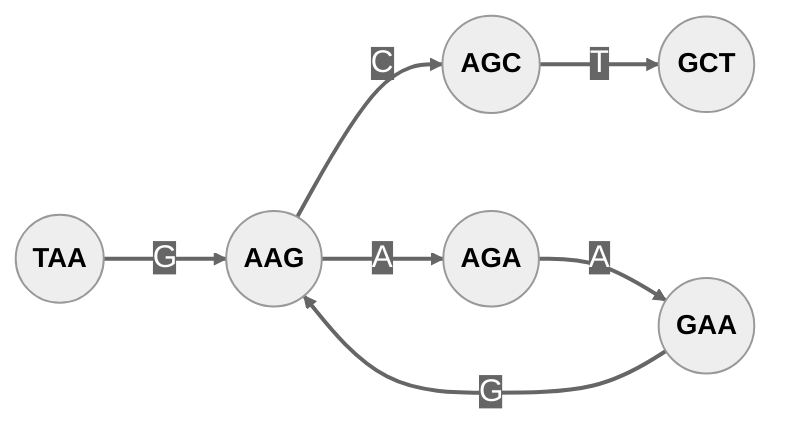
\includegraphics[width=0.6\textwidth]{images/EulerianPath.png}
  \caption{An example of a DBG with $k = 3$ where one can trace a perfect Eulerian path. This path is $TAAGAAGCT$.}\label{fig:EulerianPath}
\end{figure}

From Figure~\ref{fig:EulerianPath}, some properties of its graph can also be pointed out, relating to contigs and unitigs, the former of which was discussed in Section~\ref{sec:Biology}.
For example, the contigs which pass through the nodes $\mathit{TAA} \rightarrow \mathit{AAG} \rightarrow \mathit{AGC} \rightarrow \mathit{GCT}$ can be seen, and the other contig would be the path $\mathit{TAA} \rightarrow \mathit{AAG}$ and $\mathit{AGA} \rightarrow \mathit{GAA}$.
However, none of these are unitigs, because the paths to these contigs branch at the vertex \textit{AAG}.
In this example, one can find the unitig paths $\mathit{TAA}$, $\mathit{AGA} \rightarrow \mathit{GAA}$, $\mathit{AGC} \rightarrow \mathit{AGC}$.
Hence, a unitig is defined as a maximal path with no branching nodes, that is, for all $v_i$ in the path of size $n$, $out_v(v_i) = 1, i = 0,\ldots,n - 2$ and $in_v(v_j) = 1, i = 1,\ldots,n - 1$~\cite{Themisto}.
For the purposes of this text, in Section~\ref{sec:Pseudoalignment}, contigs will not be of use, but unitigs are an important concept and they will further expanded on.

For the SBWT~\cite{SBWT}, which is discussed in Section~\ref{sec:SBWT}, and thus also for this thesis, each node must have at least one incoming node.
To solve this, the nodes without an incoming node, that is, all vertices where $\#in(v_i) = 0$, are taken, and a new node which has the first character a \textit{\$} symbol is added, and the rest of the characters are the first $(k-1)$ characters of the sequence corresponding to the original node.
As an example of these nodes, given a node without any incoming edges corresponding to the $k$-mer $AAT$, one would add a new node $\$AA$.
Recursively, another node is added in the same manner to the new node.
The base case is when the final node which has $k$ $\$$-symbols is added.
Therefore, in the case of the previous example, the nodes $\$\$A$ and $\$\$\$$ are also added.

This means that the alphabet size is now 5: \textit{ACGT} and \textit{\$}.
However, make an important mental note that the nodes never point to another node whose corresponding sequence ends with a $\$$-symbol, that is, no edge will ever contain a $\$$-symbol as a label.
The only sequence which ends with a $\$$-symbol is $\$\$\$$, and this is the only node that does not have any incoming edges.
Thus, it will be seen that there is no need to worry about the expanded alphabet size later on, due to this property.
The altered results from Figure~\ref{fig:FastaqToDbg} are found in Figure~\ref{fig:FastaqToDbgWithDollars}.

\begin{figure}[t]
  \centering
  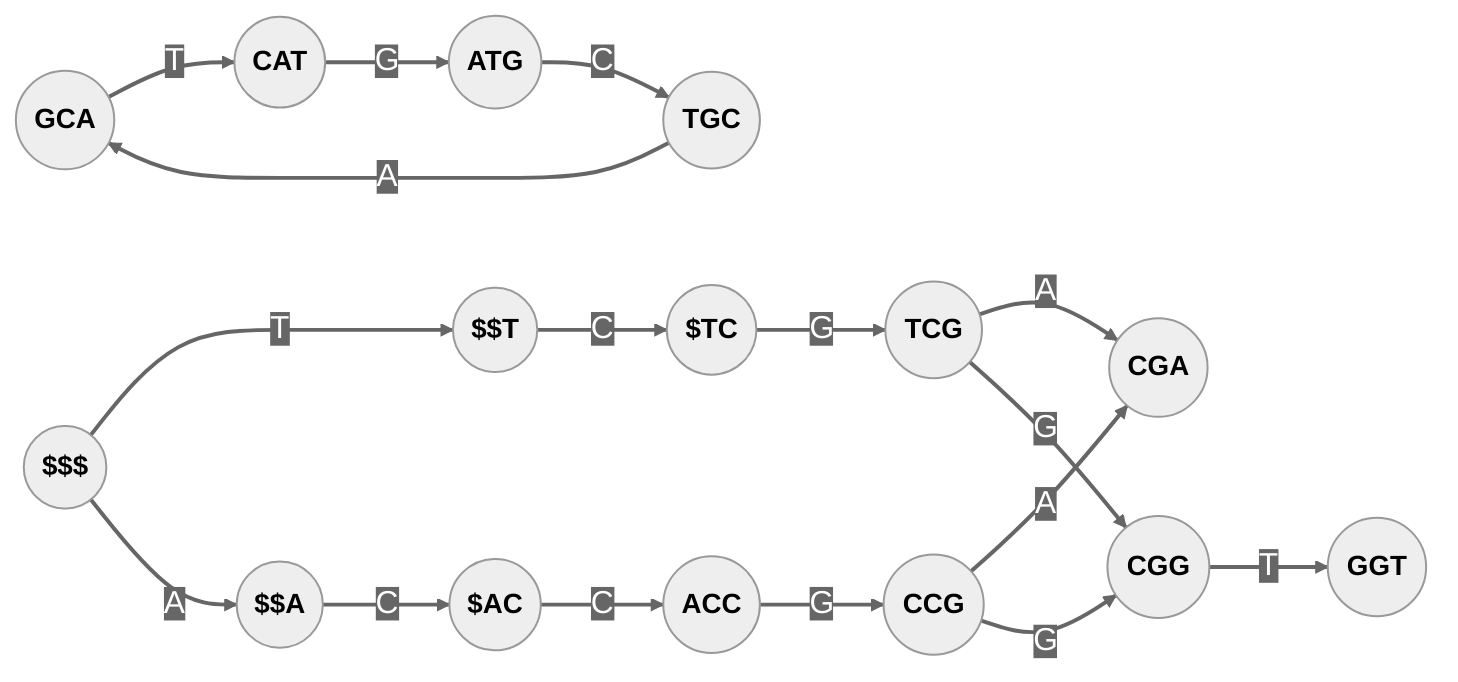
\includegraphics[width=\textwidth]{images/FastaqToDbgWithDollars.png}
  \caption{The altered DBG from Figure~\ref{fig:FastaqToDbg} where extra $\$$ nodes are added to existing nodes with no incoming edges with extra \$-symbols.}\label{fig:FastaqToDbgWithDollars}
\end{figure}


\section{Spectral Burrows Wheeler Transform}\label{sec:SBWT}

Succinct data structures are those which represent the necessary data close to its information-theoretic bound while still allowing fast searches within it~\cite{Succinct}.
The Spectral Burrows Wheeler Transform (SBWT)~\cite{SBWT} represents the DBG as a succinct data structure.
In this case, it represents it as a collection of bit vectors.
The first to do this were the authors of BOSS~\cite{SuccinctDeBruijnGraphs}, but the authors of SBWT managed to create a data structure where searching for the index of a $k$-mer takes $O(k)$~\cite{SBWT}.
In this section, the construction of this structure is discussed, as well as how to use it, and its limitations.
One limitation will be mentioned now to make sure the reader does not get confused while reading.
This data structure only guarantees searches for $k$-mers of fixed size.
This means that if the data structure was built with $k=31$, then it will only support queries for $k$-mers of size $k=31$ or less.

\subsection{Construction}

In this subsection an SBWT structure will be built.
Although the name implies that a Burrows Wheeler Transform (BWT)~\cite{BWT} is used for this succinct data structure, the similarities are distant enough that it is possible to explain the SBWT without going into details of the BWT.\@
Figure~\ref{fig:SbwtConstruction} shows the entire construction pipeline in a single figure, so it is good to refer to it while reading the rest of this section.
The first step is to extract all $k$-mers and reverse complements and create a DBG where an edge $a \rightarrow b$ is drawn for every $k$-mer $a$ and $b$ where the $k-1$ suffix of $a$ is equal to the $k-1$ prefix of $b$.
For example, given $k=3$ and the $k$-mers \textit{ACG, CGA}, and \textit{CGT}, edges $ACG \rightarrow CGA$ and $ACG \rightarrow CGT$ are created, because the $k-1=2$ suffix of \textit{ACG} is equal to the $k-1=2$ prefix of the other two $k$-mers.
The necessary $\$$ $k$-mers are then added to this DBG.\@

Next, the $k$-mers are sorted in ascending colexicographic order.
Colexicographic order means that to get the weight of the string, the reverse of the string must be considered.
After reversing, the  strings can then be sorted in ascending lexicographic/alphabetic order.
The $\$$ character is always weighted as smaller than all the other characters when sorting, meaning that the alphabet, in ascending order, is $\$ACGT$.

From the DBG, the labels of the outgoing edges are extracted and associated with the sorted $k$-mers.
These are then collapsed, such that only the first $k$-mer with a unique suffix of size $k-1$ has outgoing edges.
The collapse is a union, or, since edges with the same $k-1$ suffix will always have the same outgoing edges due to the DBG construction step, one can simply set the outgoing edge label set of the other nodes as the empty set $\emptyset$.
After collapsing, the edge labels column can be replaced with 4 bitvectors, one for each character.
Notice that no edge can ever have a $\$$ symbol, so there is no need for 5 bitvectors, even though the alphabet size is 5.
A cumulative sum map is also created, which is labeled as the c-map.
This stores the cumulative sum of the bit vectors, starting from 1 and then adding up each bit vector for each letter in ascending order.

\begin{figure}[t]
  \centering
  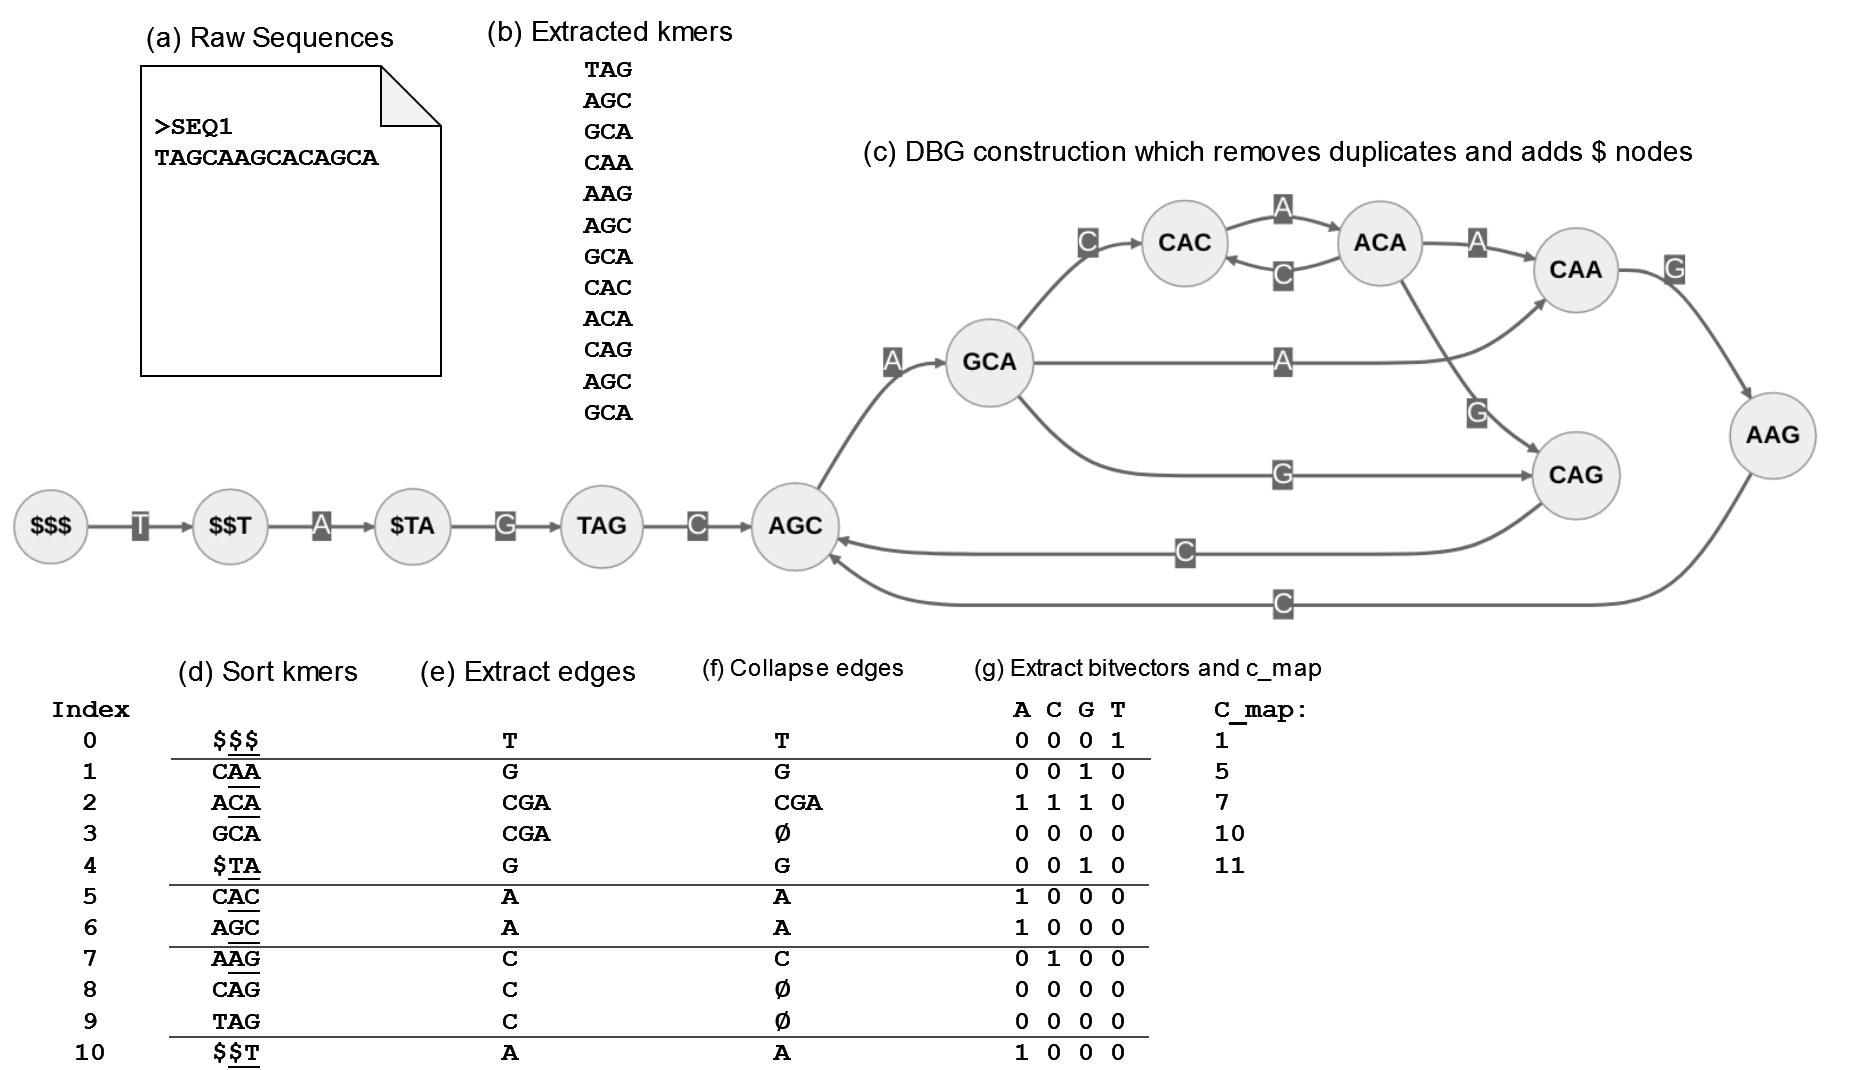
\includegraphics[width=\textwidth]{images/SbwtConstruction.png}
  \caption{SBWT construction pipeline. Note that for this example, the reverse complements are omitted for simplicity and clarity. The first edge is underlined in the sorted lists with unique $k-1$ prefixes.}\label{fig:SbwtConstruction}
\end{figure}

\subsection{Querying}\label{sec:SBWTQuerying}

For querying, one can use a technique similar to a BWT query~\cite{BWT}.
Remember that the only queries which can be done are for $k$-mers of size $k$ or less, that is, the same $k$ used in construction.
The notation will first be defined informally with an informal traversal example, before formally defining the efficient algorithm for traversal.

For the examples, the same construction from Figure~\ref{fig:SbwtConstruction} will be used.
In this figure, long gray lines indicate where the $k$-mers associated with one character begins and where those associated with the previous character ends in the sorted list.
Let $k$-mers associated with a character $c$ mean that the last character of the $k$-mer is $c$.
The list of $k$-mers associated with a character $c$ is $K_c = [k_1, k_2, \ldots, k_{c_{\max}}]$.
To search, two pointers are kept track of, a \textit{left} pointer and a \textit{right} pointer.
In the context of the figure, left means top, and right means bottom.
The algorithm shifts these two pointers around until they meet if the $k$-mers exist, or until the left pointer is greater than the right pointer, in which case it means that the $k$-mer was not found.
These pointers are concerned with the collapsed edges list, so look at these while going through the example.
The informal pseudo code is given in Algorithm~\ref{alg:IndexSearchInformalPseudoCode}, and the formal pseudo code will be discussed next and is then summarised by Algorithm~\ref{alg:IndexSearchFormalPseudoCode}.

\begin{algorithm}
	\KwIn{\newline
    A sequence $S = c_1, c_2, \ldots, c_k$ \newline
    The list of collapsed edges \newline
		The list of indexes where each $k$-mer set associated with one character starts and ends\newline
	}
	$\mathit{left}$ = index of first $k$-mer associated with $c_1$

	$\mathit{right}$ = index of last $k$-mer associated with $c_1$

	\ForEach{c \textbf{in} S[2 \ldots $k$]}{
    $\mathit{left}$ = index of first $k$-mer associated with $c$ + number of characters $c$ up to this pointer in the collapsed edges list ($\mathit{left}$), the index of this pointer not included

    $\mathit{right}$ = index of first $k$-mer associated with $c$ + number of characters $c$ up to this pointer in the collapsed edges list ($\mathit{right}$), the index of this pointer included \-- 1

    \If{$\mathit{left}$ > $\mathit{right}$}{\
      \textbf{return} not found
    }
  }
  \textbf{return} $\mathit{left}$ \textit{// or }$\mathit{right}$\textit{, they will have the same value}
	\caption{Index Search function (Informally Defined)}\label{alg:IndexSearchInformalPseudoCode}
\end{algorithm}

This next part will go through a full example search for the sequence $\mathit{CAC}$, which is know to exist in the dataset.
While doing this example, the reader is invited to look at Figure~\ref{fig:IndexQueryExample} for a visual representation of the movement of the left and right pointers.
The first character is $C$, so the algorithm starts by placing the pointers at the start and end of the $k$-mers associated with the character $C$, that is, indexes 5 and 6 for the left and right pointers respectively.
The next character is $A$, so the algorithm performs a check for how many $A$s there are in the collapsed edges list, until it gets to each of the left and right pointers, with the exception that for the left pointer, the $A$ at the index of this pointer itself is not included.
Thus, for the left pointer, the algorithm has a single $A$, so it moves the left pointer to the index of the $k$-mer associated with the first $A$ + 1, that is, index 2.
At index 6, including the index itself, it has three $A$s, so it moves this pointer to the index of the $k$-mer associated with the first $A$ + 3, that is, index 3.
Lastly, the right pointer must be moved one index downwards, so now it is at index 2, same as the left pointer.

\begin{figure}[t]
  \centering
  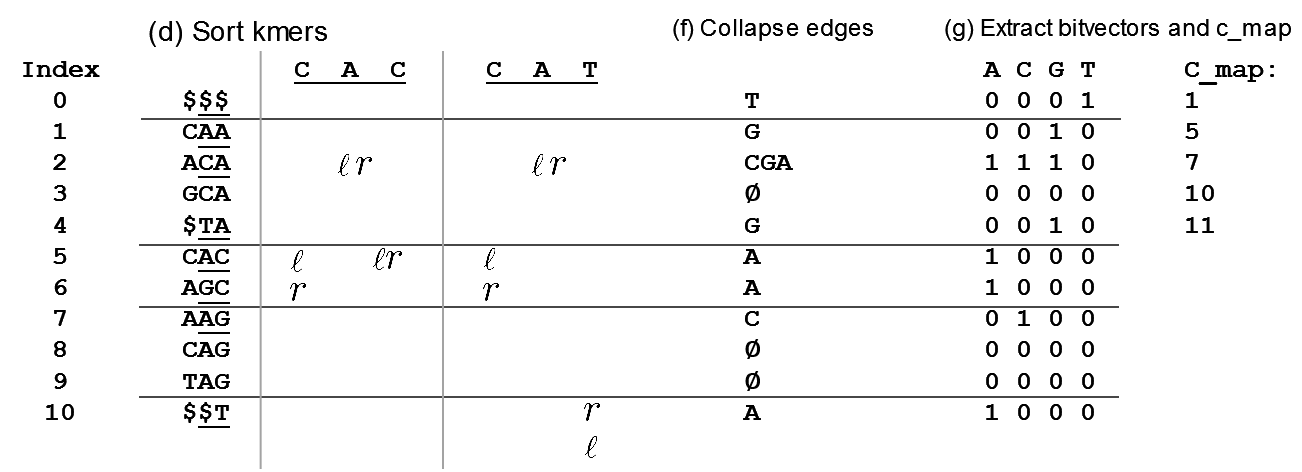
\includegraphics[width=\textwidth]{images/IndexQueryExample.png}
  \caption{Two examples of querying through the SBWT structure created in Figure~\ref{fig:SbwtConstruction}. The sequences $CAC$ is searched, which is found, and $CAT$ is not found.}\label{fig:IndexQueryExample}
\end{figure}

Lastly is the character $C$ again.
At the left pointer, up to this point there have been no $C$s in the collapsed edge list, so the pointer is moved to the index of the $k$-mer associated with the first $C$, that is, index 5.
Including the index at the right pointer, a single $C$ has been seen, so the pointer is moved to the index of the first $C$ + 1, to index 6, and then move one index backwards, to index 5.
The algorithm has now reached the end of the string, and the left and right pointer are equal and are both at index 5, which means that the index of the $k$-mer $CAC$ in the SBWT is 5.
By looking at the sorted $k$-mer list again, this claim may be verified.
The reader is encouraged to try this with other $k$-mers as well.

In the end of a $k$-mer query, the left and right pointer will always be equal, if the $k$-mer has been found.
This works because the $k$-mers are sorted and the edges are collapsed.
When the edges are collapsed, the algorithm is essentially making sure that in the DBG, each edge only has a single incoming node~\cite{SBWT}, as seen in Figure~\ref{fig:PrunedDBG}.
Next is an example using the same technique, but for a $k$-mer not present in the dataset.

\begin{figure}[t]
  \centering
  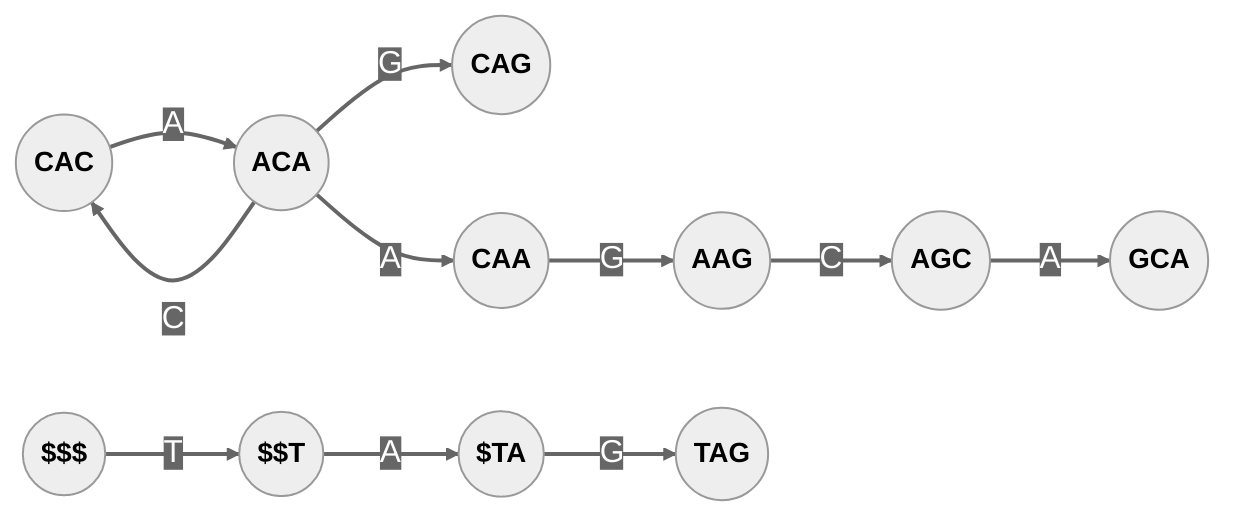
\includegraphics[width=\textwidth]{images/PrunedDbg.png}
  \caption{Pruned DBG from figure~\ref{fig:SbwtConstruction}}\label{fig:PrunedDBG}
\end{figure}

Now the sequence $\mathit{CAT}$ is considered.
Following from the previous example, both of the pointers will be at index 2 after considering both characters C and A.
Now put the left pointer at the index associated with the first $T$ + the number of $T$s seen thus far, which is $10 + 1 = 11$.
Similarly, the right pointer is put in the same location \-- 1, that is, at index 10.
Now, the left pointer is greater than the right pointer, so the algorithm will return that the $k$-mer has not been found.
Figure~\ref{fig:IndexQueryExample} also shows this example visually.

Now comes the definition for how one can do these queries algorithmically and in an efficient manner.
Notice that by using the c-map, one can know where the first $k$-mer associated with each character is.
The first element of this map is always 1, due to the node containing $k$ $\$$s.
Then, using the bitvectors for each character, the number of characters that exist up to that point in the collapsed edge list can be known, by counting the number of 1s.
To count the number of 1s, the algorithm uses what is known as the rank function for bitvectors.
Thus, $rank(b, i)$ gives the number of 1s for the bitvector $b$  up to but not including the index $i$.
For example, given $b=010110$ in binary, $rank(b, 0) = 0, rank(b, 1) = 0, rank(b, 2) = 1, rank(b, 3) = 1, rank(b, 4) = 2, rank(b, 5) = 3$ and $rank(b, 6) = 3$.
The formal definition of the algorithm can be now seen in Algorithm~\ref{alg:IndexSearchFormalPseudoCode}.

\begin{algorithm}
	\KwIn{\newline
    A sequence $S = c_1, c_2, \ldots, c_k$ \newline
    Bitvectors $b_A, b_C, b_G, b_T$
    c-map $C$
	}
  $\mathit{left}$ = $C[c]$

  $right$ = $C[c+1]$\--1  \textit{// C[A] = C[0], C[C] = C[1], \ldots}

	\ForEach{c \textbf{in} S[2 \ldots $k$]}{
    $\mathit{left}$ = $C[c]$ + rank ($b_c$, $\mathit{left}$)

    $right$ = $C[c]$ + rank ($b_c$, $\mathit{right} + 1$) \-- 1

    \If{$\mathit{left}$ > $\mathit{right}$} {\
      \textbf{return} not found
    }
  }
  \textbf{return} $\mathit{left}$
  \caption{Index Search function (Formally Defined)}\label{alg:IndexSearchFormalPseudoCode}
\end{algorithm}

Note that since $i$ itself is not included, $\mathit{rank}(0) = 0$ always holds.
Some other material may define this rank function a bit differently, such as including the 1s at index $i$, however, in this thesis, it is defined this way in order to stay true to the implementation.
This is also the implementation used by $sdsl$~\cite{SDSL}, which is a popular bitvector manipulation library.
Knowing all this, one can view the c-map as a cache for cumulative bitvector sums (+1), which means that when storing the SBWT, only two items are needed: the bitvectors, and the value for $k$, as everything else can be recomputed.

The heaviest part of this algorithm is the rank function.
Counting the number of 1s from the start of the bitvector at each step would be extremely inefficient.
On the previous CPU implementation of Themisto~\cite{Themisto}, the SDSL~\cite{SDSL} rank function is used.
Meanwhile, on the previous GPU implementation~\cite{Harri}, the Poppy data structure~\cite{Poppy} is used, to turn the rank function from $O(n)$, where $n$ is the number of vertices in the DBG, to $O(1)$, needing at most 3 cache line accesses per query.
This makes the entire search function $O(k)$.
For this thesis, Poppy is used, hence this will be further focused on.
Another advantage of this data structure is that its memory footprint is negligible, as it only uses 6.25\% more memory than the bitvector alone~\cite{Poppy}.

To construct the Poppy data structure, the vectors can be scanned once and checkpoints are inserted at each step.
For those familiar with skip lists, the cost-saving ideas are comparable.
Checkpoints are set at 3 layers.
Layer 0 stores a checkpoint every $2^{32}$ bits, so that it counts the total cumulative number of bits.
This type of cumulativeness is called absolute cumulative.
Thus, $2^{32}$ is the hyperblock size.
Layer 0 is stored as a bitvector of 64-bit integers.

Next is to construct layer 1.
This layer is similar to to layer 0 but it stores a checkpoint after $2^{10} = 1024$ bits.
$2^{10}$ is the superblock size.
Another special feature of this layer is that it resets to 0 once it reaches one of the layer 0 checkpoints, that is, once the number of bits it has covered reaches the hyperblock size, it restarts from 0.
This gives it the feature that layer 1 counts will always have a maximum size of $2^{32}$, and thus can be stored in 32-bit integers.

Lastly is layer 2, which sets a checkpoint after every $2^8 = 256$ bits, or after every $4 \times 64$ bits.
$2^8$ is the basicblock size.
This layer is not cumulative at all, unlike the previous two layers, where layer 1 is relative cumulative and layer 0 is absolute cumulative.
The maximum value for layer 2 is $2^8$, which means that for each value, they only need 8 bits.
Layer 3 could be considered to be the bitvector itself.
The full data structure is shown in the first part of Figure~\ref{fig:Poppy}.

\begin{figure}[t]
  \centering
  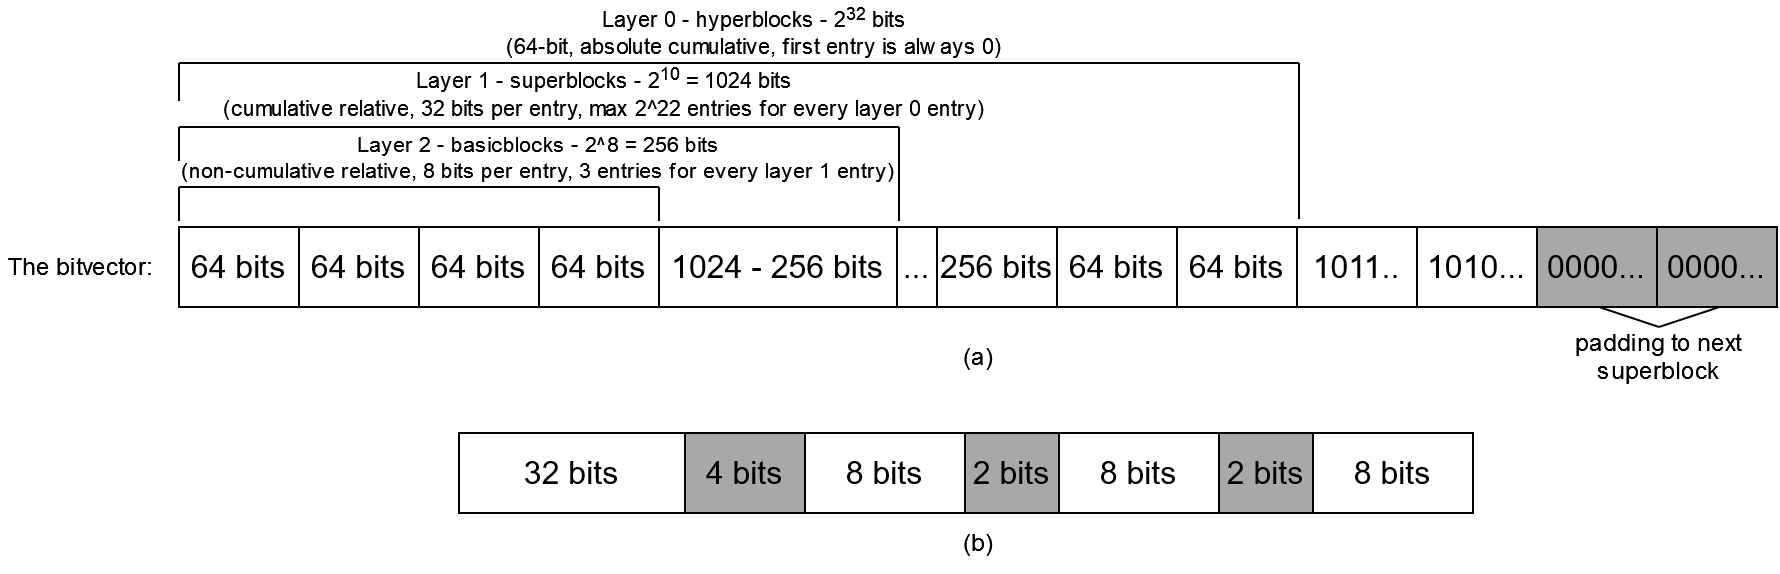
\includegraphics[width=\textwidth]{images/Poppy.png}
  \caption{(a) Poppy data structure fully constructed, with padding shown to the next superblock. (b) The combined storage representation for layer 1 and layer 2.}\label{fig:Poppy}
\end{figure}

Then, to query, one would need to first obtain the previous layer 0 entry, which always has a 0 entry at the start for convenience.
This entry is then added to the previous layer 1 entry, which also has a 0 entry at the start.
The result would then need be added to the previous layer 2 entries within the same superblock.
Lastly, the rank of the integers within the same basicblock is added up until the index needed for the rank function.

The storage of layers 1 and 2 can be combined in a single 64-bit integer, so the data structure can have a layer 1 entry and the inner layer 2 entries.
This is shown in the second part of Figure~\ref{fig:Poppy}.
As a result of this optimisation, the algorithm may need to do more bit shifting in order to obtain the values for layers 1 and 2, however the values in these layers can be accessed with a single memory access, which is usually a bigger bottleneck than bit shifts.
The big advantage of this data structure is that it can handle vectors up to $2^{64}$ bits, which is the maximum that the algorithm as a whole can handle.

This concludes the SBWT section.
Note, again, that this algorithm guaranteed to find $k$-mers of the size of the same $k$ with which the algorithm was built for, or less.
As such, $k$ should be as large as possible, if accuracy is the goal.
However, the larger the $k$, the larger the memory footprint of the index, so it is not recommended to go overboard.
$k=31$ is a usual choice, as the entire query can fit into a single 64-bit integer by bit packing ACGT into 2 bits each, though this technique is not used by the implementation for this thesis, which is in Section~\ref{sec:Phase1}.
$k$ is taken to be 31 since this is an odd number and palindromes should be avoided, as discussed earlier.
The disadvantage of this data structure is that information is lost as to where the $k$-mer originated from, if the input consists of multiple reads, or multiple files.
The next section will describe how additional labels, known as colors in this domain, can be added to the vertices in the DBG in order to determine where the $k$-mers originate from.


\section{Pseudoalignment}\label{sec:Pseudoalignment}

\subsection{Background}

To start describing pseudoalignment, colored DBG must be described first~\cite{CDBG, SuccinctColoredDeBruijnGraphs}.
Throughout this chapter and beyond, the terms $u64$, $u8$, and other variants may be used.
$u64$ means an unsigned 64-bit integer, whereas $u8$ means an unsigned 8-bit integer, and so on for other values of this format.
Lets take a look at Figure~\ref{fig:FastaqToCdbg}.
Say that you are given 2 sequences $S_1$ and $S_2$ with $k$-mer sets $K_1 = a_1, a_2, \ldots, a_n$ and $K_2 = b_1, b_2, \ldots, b_m$.
Now each sequence is given a label, usually some u64.
If a $k$-mer belongs to a sequence, the $k$-mer is marked with the same label as the sequence.
Moreover, if a $k$-mer belongs to multiple sequences, it is marked with the label of that sequence.
These labels are the colors.
Implementation-wise, these colors are represented as simple u64s, so each $k$-mer has a set of u64s associated with it~\cite{Themisto}.

\begin{figure}[t]
  \centering
  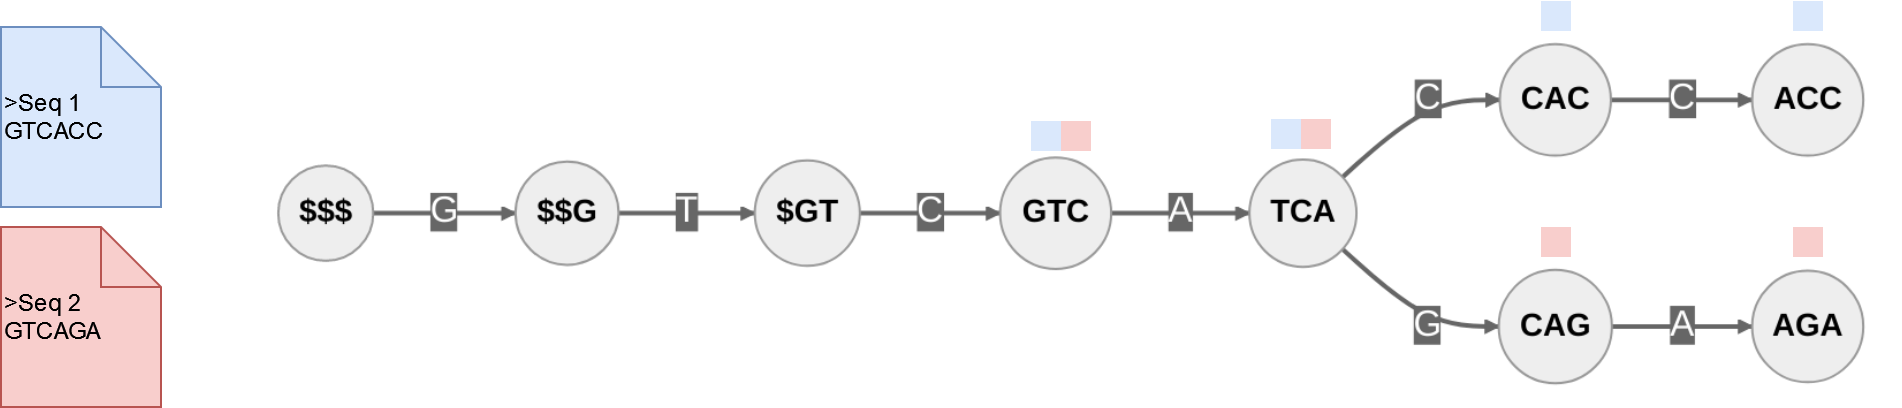
\includegraphics[width=\textwidth]{images/FastaqToCdbg.png}
  \caption{Transforming FASTA/FASTQ files into a colored DBG with $k=3$. Reverse complements are not included in this example.}\label{fig:FastaqToCdbg}
\end{figure}

Different sequences may have the same color.
One use of this is to group the sequences of a single reference genome and say they all have the same color.
This way, if a $k$-mer is labeled with the color of a reference genome, it is known that the $k$-mer is found in that genome.
Then, if all the color sets of all $k$-mers of a read contain the same color, that is, the intersection of all the color sets has a color, one may say that the read is found in the reference genome associated with that color.
If a $k$-mer is not found in the DBG, then it is ignored.
This is the technique used by Kallisto~\cite{Kallisto}, the first pseudoalignment tool.

Metagraph~\cite{Metagraph} and Bifrost~\cite{Bifrost}, two separate pseudoalignment tools, went one step further than Kallisto and instead of ignoring the $k$-mers not found in the DBG, they set a threshold $\tau$, and if more than $\tau$ color sets of $k$-mers in a read include a color, then it is said that the read is associated with that color.
Themisto~\cite{Themisto}, whose implementation this work is based on, combines the two methods so that the user can choose to remove or include the $k$-mers with no color sets, and then set a threshold on the remaining $k$-mers.
If a threshold $\tau=1$ is set and the missing $k$-mers are ignored, then the result is the same as Kallisto.
Meanwhile, if the missing $k$-mers are included, the results are the same as those of Metagraph and Bifrost~\cite{Themisto}.
Themisto has shown to be the best method as, besides supporting both threshold and the removal of missing $k$-mers, it is usually faster and uses less space than other methods~\cite{Themisto}.
Metagraph has the potential of using less memory for its index when using binary-relation wavelet trees, but then has 100 times less query throughput on some datasets~\cite{Themisto}.

When doing pseudoalignment, a DBG is usually built out of the $k$-mers of many reference genomes, and each $k$-mer is given the colors of all genomes it belongs to.
Thus, there are as many colors as genomes within this DBG.
However, if the dataset has hundreds of thousands of genomes, it may be a good idea to group some of them together, thus avoiding having too many colors, as this may lead to intense memory requirements and processing times, especially if each $k$-mer has its own color set.
Pseudoalignment works because it was found that it is often not necessary to know in which position a read was within a genome to attribute it to a genome, only which genome it originated from~\cite{Kallisto}.

\subsection{Themisto}

Now, the construction and optimisations of the colored DBG as used in Themisto~\cite{Themisto}, which uses GGCAT~\cite{GGCAT} for colored unitig construction, will be discussed.
Firstly, there is no need to keep a color set for every $k$-mer.
Rather, certain conditions can be identified where the $k$-mers must have an associated color set, and for the rest of the $k$-mers the algorithm would need to move forward in the graph until the next $k$-mer which has a color set.
If two $k$-mers have the same color set, they can point to the same memory position, rather than duplicating the colors, hence avoiding doubling memory requirements.
The $k$-mers with a color set associated with them are called key-$k$-mers.
The conditions for a vertex to be labeled as a key-$k$-mer, and therefore must have a color set associated with it, are described next, and visualised in Figure~\ref{fig:KeyKmers}.
Reference is made to this figure as each condition is described.

The first condition out of four for being a key-$k$-mer is if it is outgoing to another vertex which is the first $k$-mer from a reference sequence.
This condition causes the vertex with $k$-mer \textit{CTT} to be a key-$k$-mer.
The second condition is if it is the last $k$-mer of a reference sequence.
This condition causes $k$-mers \textit{CCT, CGG} and \textit{GAG} to be key-$k$-mers.
Third, if it has an outgoing edge to a vertex $v_i$ with $\#in_v(v_i) \ge 2$.
Because of this, \textit{TAC} and \textit{AAC} are labeled as key-$k$-mers.
Fourth and last, if the vertex $v_i$ itself has $\#out_v(v_i) \ge 2$.
The last condition causes \textit{TCG} to be labeled as a key-$k$-mer.
Notice how each unitig will have the same color set, unless a new sequence starts in the middle of that unitig.

Remember that these rules exist because one can always go forwards in the graph, using Algorithm~\ref{alg:MovingForward}, but not backwards.
This algorithm assumes a single outgoing edge from the current vertex, otherwise, it would lead to ambiguities.
The less steps needed, the better, because for each step in the graph walk that needs to happen requires a random read, since the $k$-mers are not ordered by their position in the graph, but colexicographically based on their $k$-mers.
As a result, ideally, every vertex would be a key-$k$-mer, which means that the color set for each $k$-mer would be stored.
However this causes too much memory to be used, as it would be necessary to store a pointer for each $k$-mer.
Hence why checkpointing is used, with a parameter $d$, where every d $k$-mers of a uniquely colored unitig becomes a key-$k$-mer.
If $d=1$, this means that every $k$-mer is a key-$k$-mer.
In Chapter~\ref{ch:Results}, the datasets used for this thesis are evaluated with $d=1$ and $d=20$.

\begin{figure}[t]
  \centering
  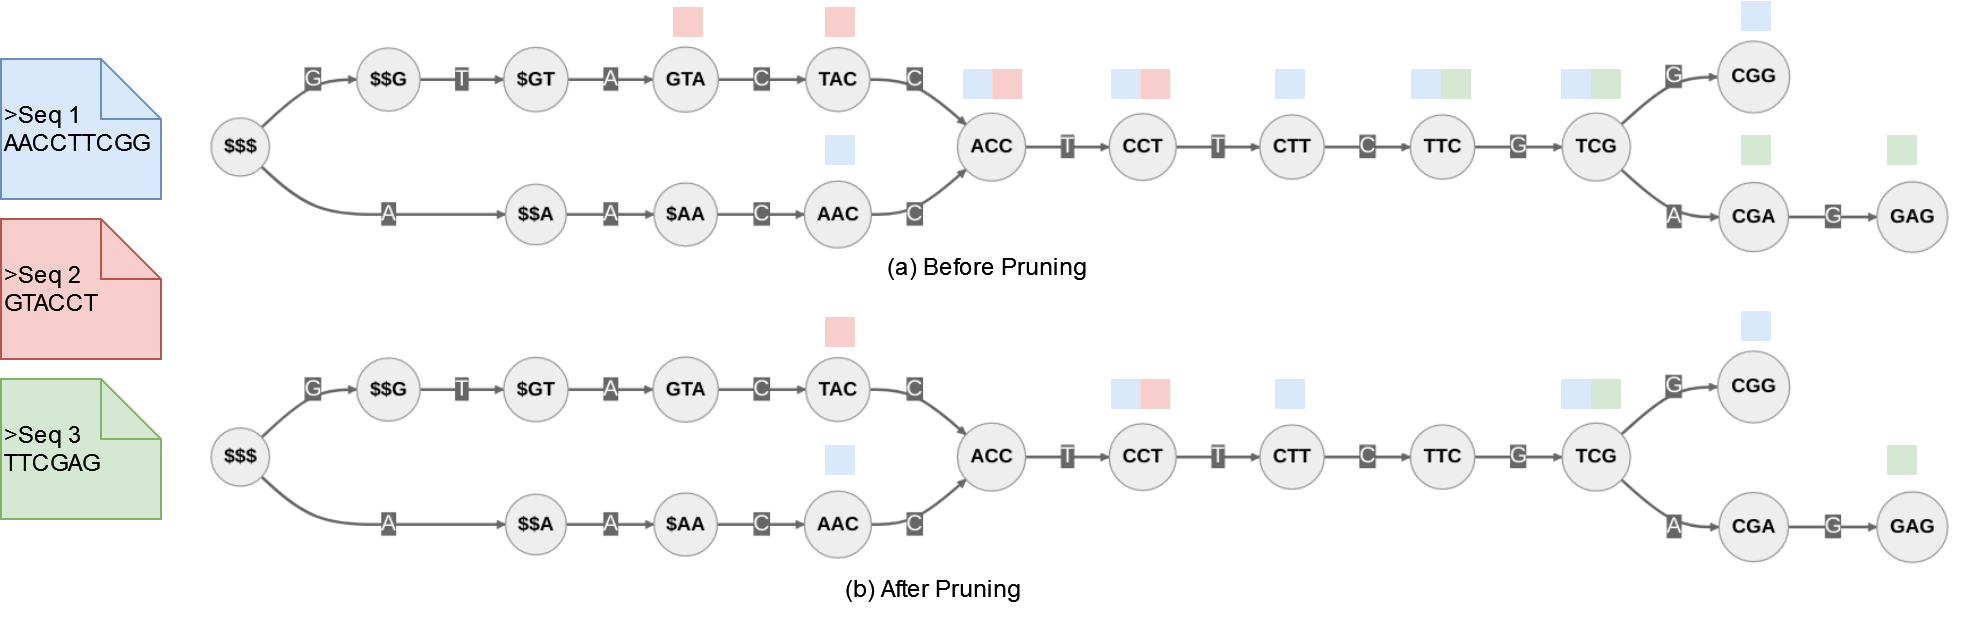
\includegraphics[width=\textwidth]{images/KeyKmers.png}
  \caption{Transforming FASTA/FASTQ files into a colored DBG with $k=3$ and then pruning it for key-$k$-mers. Once more reverse complements are omitted for simplicity of the example, but these would be included also in practice.}\label{fig:KeyKmers}
\end{figure}

\begin{algorithm}
	\KwIn{ \newline
    The current index $i$ \newline
    Bitvectors $b_A, b_C, b_G, b_T$ \newline
    c-map $C$
	}

  \ForEach{$b, label$ \textbf{in} $Bitvectors, BitvectorLabels$}{\
    \If{$b[i]$ = 1}{\
      \textbf{return} $C[label]$ + rank($b_{label}, i$)
    }
  }
	\caption{Walking 1 step forward in the SBWT}\label{alg:MovingForward}
\end{algorithm}

Next the color set storage in Themisto is discussed.
Figure~\ref{fig:ColorComponents} contains a visualisation of each of the components which makes up the whole color structure.
First is a bitvector indicating the key-$k$-mers, the \textit{key\_kmer\_marks}, where a 1 at index $i$ indicates that the vertex at index $i$ corresponds to a key-$k$-mer.
The length of this bitvector is the same length as the number of vertices.
Next, there is the color set indexes \textit{color\_set\_idxs}, which are integers that point key-$k$-mers to the index of the color set they are associated with.
Additionally, a bitvector of the same size of the \textit{key\_kmer\_marks} indicates how the color set for that $k$-mer is stored, the \textit{is\_dense\_marks}.

Themisto uses an adaptive color set storage method which allows it to save a lot of space, which is called the \textit{hybrid} technique.
Using this method, there are two ways a color set can be stored: dense or sparse.
The dense method stores color sets as bitvectors, where a 1 indicates that the color at that index is present.
Any trailing 0s are truncated as an optimisation.
The bitvectors for the dense color sets are stored contiguously in a large bitvector called the \textit{dense\_arrays}.
Thus, another vector of unsigned integers is necessary, to indicate at which bit each color set starts and ends, called the \textit{dense\_arrays\_intervals}.
This array has a final unsigned integer at the end that has the end of the last vector, which would be the start of the next bitvector if it existed.
A compact vector of unsigned integers is used.
Compact means that the vector uses only as much memory as needed, by using $\lceil log_2(n) \rceil$ bits per character, where $n$ is the largest index.
The sparse format then uses compact vectors to store the color set indexes which are present in a color set, the \textit{sparse\_arrays}.
Similarly to the dense format, the sparse vector is stored contiguously, so another compact vector is used to store the start indexes, dubbed as the \textit{sparse\_arrays\_intervals}.
Each sub-array in the \textit{sparse\_arrays} is sorted, to make querying and therefore intersecting the color sets of reads later easier.

\begin{figure}[t]
  \centering
  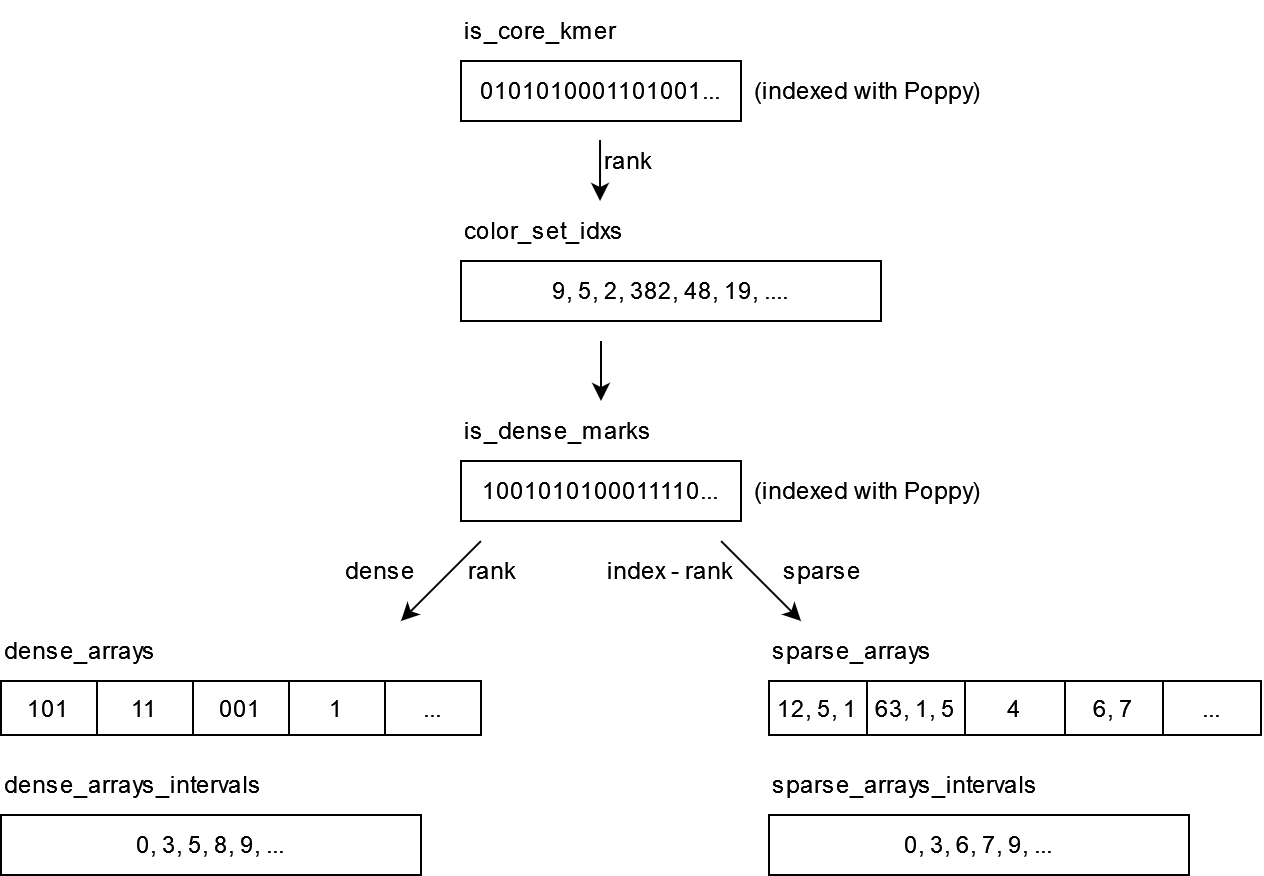
\includegraphics[width=0.85\textwidth]{images/ColorComponents.png}
  \caption{A visualisations of all components used for color storage and some hints for searching. Note that all non-bitvector arrays are compact unsigned integer vectors.}\label{fig:ColorComponents}
\end{figure}

Algorithm~\ref{alg:ColorSearch} shows the color set search, given the index of a key-$k$-mer.
This corresponds to Figure~\ref{fig:ColorComponents} and the terminology used so far, which will carry on to the next section as well.
Themisto uses some optimisations for combining color sets.
For example, when $\tau=1$, a technique which is also used in Kallisto~\cite{Kallisto}, is that when both color sets that need to be combined are dense, a bitwise AND can be used.

\begin{algorithm}
	\KwIn{ \\
    The index $i$ of a key-$k$-mer in the SBWT structure

    $key\_kmer\_marks$ (indexed with Poppy)

    $color\_set\_idxs$

    $is\_dense\_marks$ (indexed with Poppy)

    $dense\_arrays$

    $dense\_arrays\_intervals$

    $sparse\_arrays$

    $sparse\_arrays\_intervals$

    $num\_colors$
	}

  $color\_set\_idx$ = $color\_set\_idxs[rank(key\_kmer\_marks, i)]$

  $is\_dense$ = $is\_dense\_marks[color\_set\_idx]$

  $is\_dense\_rank$ = rank($is\_dense\_marks, is\_dense$)

  \If{is\_dense}{\
    $start$ = $dense\_arrays\_intervals[is\_dense\_rank]$

    $end$ = $dense\_arrays\_intervals[is\_dense\_rank$ + 1]

    \textbf{return} $dense\_arrays[start, \ldots, (end - 1)]$  // returns dense format
  }\Else{
    $start$ = $sparse\_arrays\_intervals[is\_dense\_rank]$

    $end$ = $sparse\_arrays\_intervals[is\_dense\_rank + 1]$

    \textbf{return} $sparse\_arrays[start, \ldots, (end - 1)]$  // returns sparse format
  }

	\caption{Obtaining the color set given the SBWT index and the color structure components.}\label{alg:ColorSearch}
\end{algorithm}

This concludes the background chapter.
The next chapter will discuss the contributions of this thesis to massively parallelise and use all computing resources available to speed up pseudoalignment.

